\documentclass[a4paper,12pt]{article}

\usepackage{mystyle}

\usepackage{gensymb}
\usepackage{scalerel}
\usepackage{stackengine}


\graphicspath{ {images/} }


% https://tex.stackexchange.com/questions/5461/is-it-possible-to-change-the-size-of-an-arrowhead-in-tikz-pgf
\usetikzlibrary{arrows.meta}


\DeclareMathOperator{\Image}{Im}

\definecolor{pink}{RGB}{218, 3, 174}
\definecolor{violet}{RGB}{148, 0, 211}
\definecolor{green}{RGB}{0, 153, 0}
\definecolor{orange}{RGB}{255, 153, 0}
\definecolor{blue}{RGB}{5, 73, 255}


% https://tex.stackexchange.com/a/101138/135045

\newcommand\widesim[1]{\ThisStyle{%
  \setbox0=\hbox{$\SavedStyle#1$}%
  \stackengine{-.1\LMpt}{$\SavedStyle#1$}{%
    \stretchto{\scaleto{\SavedStyle\mkern.2mu\sim}{.5150\wd0}}{.6\ht0}%
  }{O}{c}{F}{T}{S}%
}}


\newcommand{\BigMiddleThree}{\;\left|\vphantom{\begin{pmatrix} 0\\0\\0 \end{pmatrix}}\right.\;}
\newcommand{\BigMiddleFour}{\;\left|\vphantom{\begin{pmatrix} 0\\0\\0\\0 \end{pmatrix}}\right.\;}


\DeclareMathOperator{\Imag}{Im}


% https://tex.stackexchange.com/questions/544453/undefined-control-sequence-after-paragraph
\renewcommand{\paragraph}[1]{\noindent\textbf{#1}\quad}


% https://tex.stackexchange.com/questions/36851/skipping-line-after-proof-in-proof-environment#comment73553_36851
\newcommand{\proofindent}{\hspace*{\fill}\par\vspace{0.5em}\noindent}


% https://tex.stackexchange.com/questions/4813/extendible-equals-sign
\makeatletter
\newcommand*{\Relbarfill@}{\arrowfill@\Relbar\Relbar\Relbar}
\newcommand*{\xeq}[2][]{\ext@arrow 0055\Relbarfill@{#1}{#2}}
\makeatother



% https://tex.stackexchange.com/a/314638/135045
\newcommand{\diff}{\mathop{}\!d\!}


% https://tex.stackexchange.com/a/22134/135045
\newcommand{\widebar}[1]{\overline{#1\mkern-1.5mu}\mkern 1.5mu}  % Needed to remove mkern trick from left side (otherwise looked not so good)




\author{Алексеев Василий}


\title{Семинар 3}
\date{16 сентября 2024}


\begin{document}
  \maketitle
  
  \tableofcontents

  \thispagestyle{empty}
  
  \newpage
  
  
  
  \vspace*{\fill}
  
  \noindent
  \emph{
    К формулировкам и доказательствам (если такие приводятся) стоит относиться критически.
    Основное в конспекте~---~решение задач (но ``критичность'' и здесь отключать не рекомендуется).
    За строгой, ясной и последовательной теорией лучше обращаться к ``нормальным'' источникам.
    (Например, к лекциям.)
  }
  
  \vspace*{\fill}
  
  \thispagestyle{empty}
  
  \newpage
  
  
  \pagenumbering{arabic}


  \section{Предел последовательности (продолжение)}
  
  Отметим несколько заметных наблюдений про сходимость последовательностей.
  
  
  \subsection{Ограниченная последовательность имеет сходящуюся подпоследовательность (теорема Больцано~--~Вейерштрасса)}
  
  \begin{figure}[ht]
    \centering
    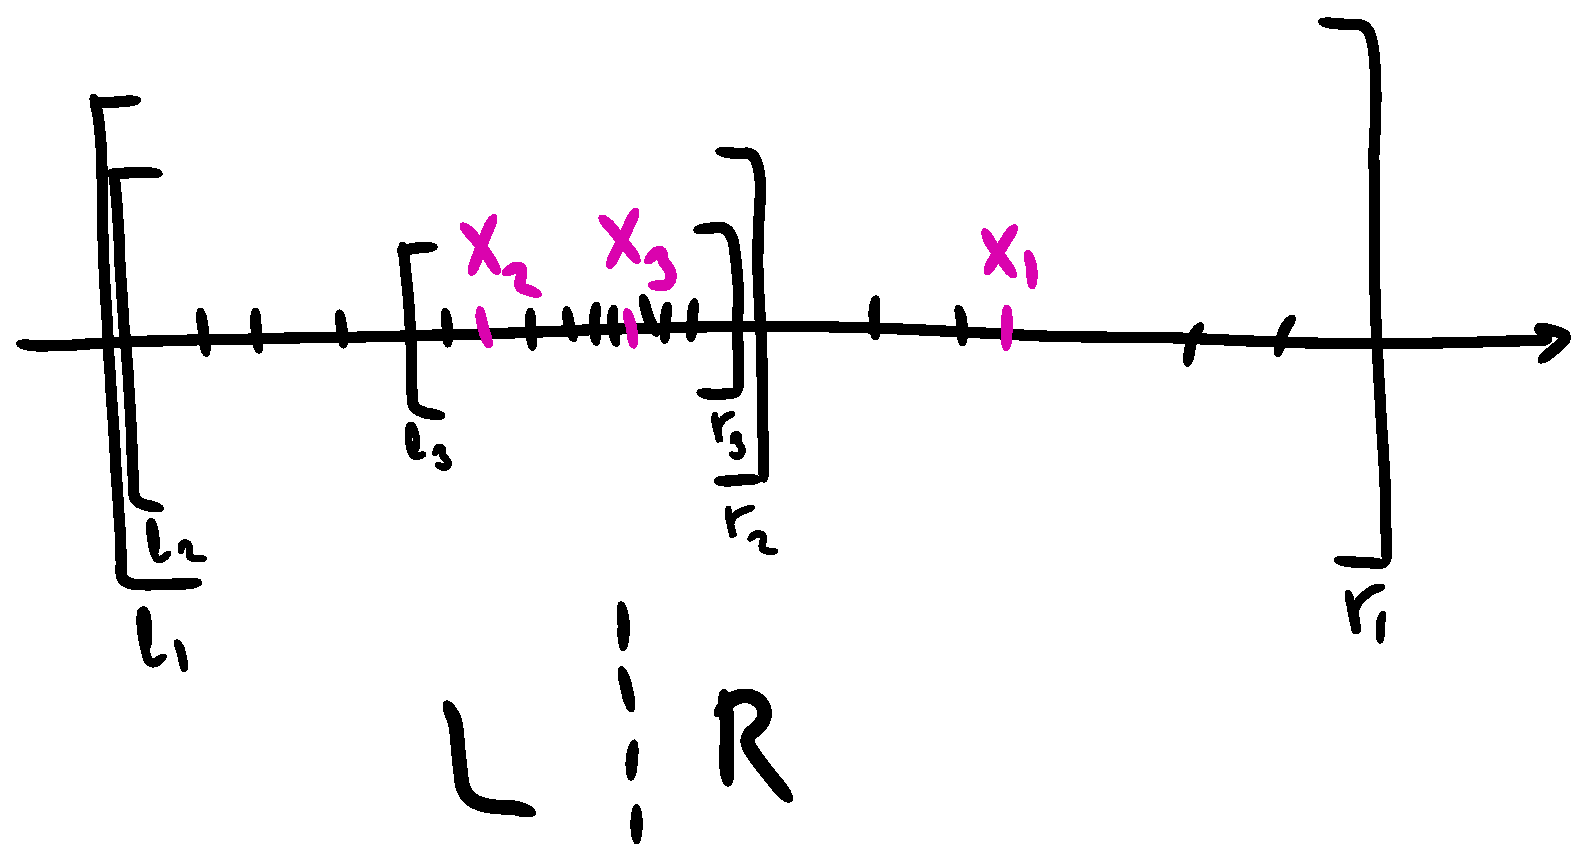
\includegraphics[width=0.6\linewidth]{images/bolcano-v}
    
    \caption{
      Из ограниченной последовательности можно выделить сходящуюся подпоследовательность.
    }
    \label{fig:bolcano-v}
  \end{figure}
  
  \begin{proof}
    Ограниченность последовательности $\{x_n\}$ равносильна тому, что все её члены лежат внутри некоторого отрезка:
    \[
      \exists C > 0\colon \forall n \in \NN \to -C \leq x_n \leq C \leftrightarrow |x_n| \leq C
    \]
    
    Убедимся в том, что есть сходящаяся подпоследовательность, просто найдя (построя) эту самую подпоследовательность~(\ref{fig:bolcano-v}).
    
    Пусть $x_1$~---~какой-нибудь элемент последовательности из отрезка~$[-C, C]$.
    Далее, поделим отрезок пополам.
    Раз бесконечная последовательность лежит на $[-C, C]$, то бесконечное число элементов будет лежать и хотя бы в одной из двух половин.
    ``Перейдём'' в эту самую половину.
    И выберем какой-нибудь $x_2$ (отличный от $x_1$, если он находится в этой же половине, и с номером, большим, чем номер элемента $x_1$).\footnote{
      $x_1$, $x_2$~---~это номера элементов как элементов строящейся подпоследовательности, то есть это ``$k$'' в индексах $\{x_{n_k}\}$.
      При этом ``оригинальные'' номера у этих элементов (как у элементов последовательности $\{x_n\}$) могли быть другими.
    }\textsuperscript{,}\footnote{
      Можно бы было немного ``заморочиться'' и описать процесс перехода к меньшему вложенному подотрезку так, чтобы он не содержал выбранный только что член подпоследовательности.
    }
    И будем повторять этот процесс: деления пополам, перехода в нужную половину и выбора очередного $x_k$ (отличного от всех выбранных ранее $x_1$, $x_2$, ..., $x_{k - 1}$).\footnote{
      На текущем отрезке $[l_k, r_k]$ всегда есть бесконечно много элементов последовательности~---~каждый раз можно будет выбрать новый элемент~$x_k$ подпоследовательности, сколько бы уже выбранных ранее элементов ни находились на этом же отрезке (их конечное число).
    }
    Что получается:
    \[
      \begin{aligned}
        &x_1 \in [l_1, r_1] = [-C, C]                        & &\bigl|[l_1, r_1]\bigr| = 2C\\
        &x_2 \in [l_2, r_2] = [-C, 0] \mbox{ или } [0, C]    & &\bigl|[l_2, r_2]\bigr| = C\\
        &x_3 \in [l_3, r_3] = [-C/2, 0] \mbox{ (например)}   & &\bigl|[l_3, r_3]\bigr| = C/2\\
        &\ldots\\
        &x_k \in [l_k, r_k]                                  & &\bigl|[l_k, r_k]\bigr| = 2C/2^{k - 1}\\
      \end{aligned}
    \]
    
    Получается \emph{последовательность вложенных отрезков} $\bigl\{[l_k, r_k]\bigr\}$, и каждый член подпоследовательности $\{x_k\}$ берётся из соответствующего отрезка.
    Последовательность отрезков стягивающаяся:
    \[
      \bigl|[l_k, r_k]\bigr| \xrightarrow{k\to \infty} 0
    \]
    (последовательность соответствующих длин отрезков стремится к нулю).
    При этом все левые концы отрезков $L \hm= \{l_1, l_2, \ldots\}$ ``очевидно'' лежат левее всех правых концов $R \hm= \{r_1, r_2, \ldots\}$.
    По аксиоме непрерывности $\RR$ чисел, найдётся точка $c$, лежащая между $L$ и $R$:\footnote{
      Вообще это объясняемое ``между делом'' утверждение о наличии общей точки у стягивающейся последовательности вложенных отрезков называется \emph{теоремой Кантора о вложенных отрезках}.
    }
    \[
      \forall l \in L,\ \forall r \in R \to l < r \quad\Rightarrow\quad \exists c \in \RR\colon \forall l \in L,\ \forall r \in R \to l < c < r
    \]
    
    Расстояние от $x_k$ до этой точки $c$, очевидно, неограниченно уменьшается по мере увеличения номера~$k$:
    \[
      |x_k - a| \leq \frac{2C}{2^{k - 1}} \xrightarrow{k \to \infty} 0
    \]
    поэтому $|x_k - a| \hm{\xrightarrow{k \to \infty}} 0$,\footnote{
      По-хорошему, это верно по теореме о двух милиционерах, о которой будет отдельно сказано несколько слов далее.
    } а значит, и $x_k \hm{\xrightarrow{k \to \infty}} a$.\footnote{
      А это тоже верно по одному из свойств сходящихся последовательностей (где про модуль), но о нём ничего сказано не будет.
    }
    
  \end{proof}
  
  
  \subsection{Ограниченная монотонная последовательность сходится (теорема Вейерштрасса)}
  
  \begin{figure}[ht]
    \centering
    \includegraphics[width=0.6\linewidth]{images/ve}
    
    \caption{
      Ограниченная монотонно возрастающая последовательность $\{x_n\}$ сходится к~$\sup \{x_n\}$.
    }
    \label{fig:ve}
  \end{figure}
  
  \begin{proof}
    Пусть, для определённости, $\{x_n\}$ монотонно возрастает.
    
    Раз последовательность ограничена, то у множества её элементов существуют конечные точная верхняя и точная нижняя грани.
    
    Монотонно возрастает, ограничена сверху числом...
    Покажем, что точная верхняя грань (которую обозначим~$M$) как раз будет являться пределом последовательности~(\ref{fig:ve}).
    Так как $M$~---~\emph{точная} верхняя грань, то любое число $M \hm- \eps$ меньше него верхней гранью являться не будет, то есть найдётся элемент последовательности $x_N$ больше него:
    \[
      \forall \eps > 0\ \exists N \in \NN\colon M - \eps < x_N
    \]
    а так как последовательность монотонно возрастает, то можно сказать и так:
    \[
      \forall \eps > 0\ \exists N \in \NN\colon \forall n \geq N \to M - \eps < x_n
    \]
    то есть все $x_n$, $n \hm\geq N$ лежат в ``левой половинке'' $\eps$-окрестности~$M$.
    
    Таким образом, $M$~---~предел $\{x_n\}$.
  \end{proof}
  
  
  \subsection{``Иногда близость означает сходимость'', или фундаментальная последовательность сходится (критерий Коши)}
  
  Из того, что последовательность $\{x_n\}$ сходится, следует, что её элементы становятся всё ближе, в том смысле что
  \begin{equation}\label{eq:fund-seq}
    \forall \eps > 0\ \exists N \in \NN\colon \forall n, k \geq N \to |x_n - x_k| < \eps
  \end{equation}
  
  Оказывается, верно и ``в другую сторону''.
  То есть можно сформулировать следующий \emph{критерий}.
  
  \begin{proposition}[критерий Коши сходимости последовательности]
    Последовательность $\{x_n\}$ сходится тогда и только тогда, когда она \emph{фундаментальна}, то есть удовлетворяет соотношению~\eqref{eq:fund-seq}.
  \end{proposition}
  
  \begin{proof}
    Из сходимости ``очевидным'' образом следует фундаментальность.
    
    Поэтому покажем, что из фундаментальности последовательности также следует её сходимость.
    Имеем, что
    \[
      \forall \eps > 0\ \exists N \in \NN\colon \forall n, k \geq N \to |x_n - x_k| < \eps
    \]
    
    Но тогда получается, что последовательность ограничена: почти все элементы лежат в $\eps$-окрестности $x_N$~(\ref{fig:all-near-xN}), конечное число элементов может лежать вне окрестности, но в любом случае  % TODO: pic
    \[
      \forall n \to |x_n| \leq C,\quad C = \max\left\{|x_N| + \eps,\; |x_1|, |x_2|, \ldots, |x_{N - 1}|\right\}
    \]
    
    \begin{figure}[ht]
      \centering
      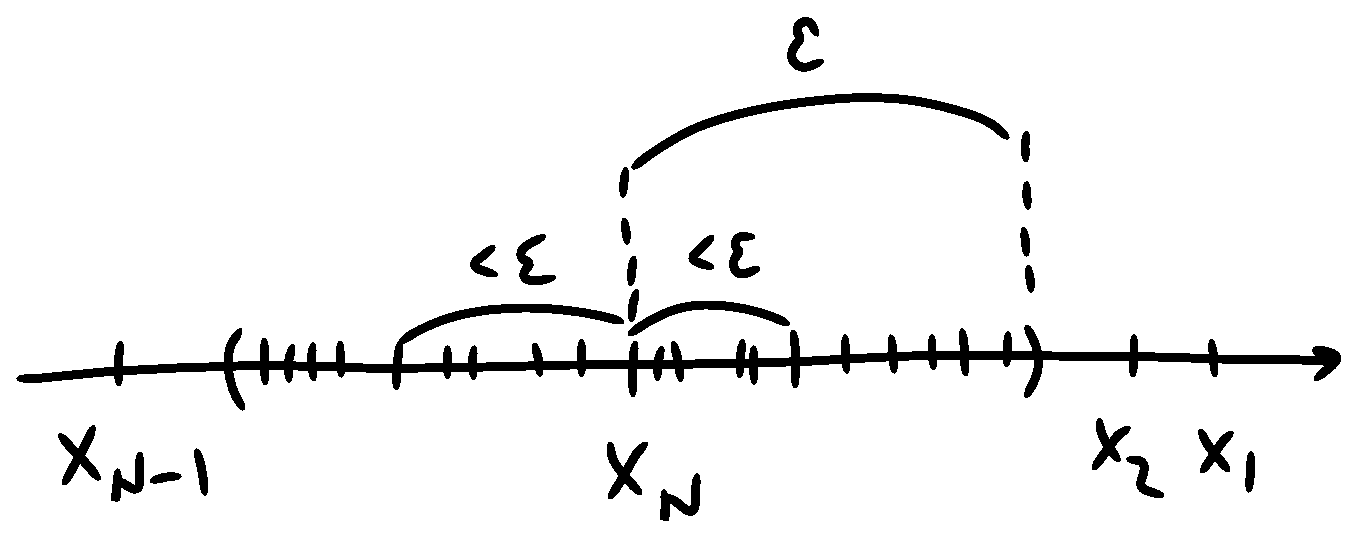
\includegraphics[width=0.6\linewidth]{images/all-near-xN}
      
      \caption{
        Фундаментальная последовательность ограничена.
      }
      \label{fig:all-near-xN}
    \end{figure}
    
    А из ограниченной последовательности, по теореме Больцано~--~Вейерштрасса, можно выделить сходящуюся подпоследовательность:
    \begin{equation}
    \begin{split}
      \exists \{x_{n_k}\} = \{y_k\}\colon \lim_{k \to \infty} y_k = a
        \leftrightarrow \forall \eps > 0\ \exists K \in \NN\colon \forall k \geq K \to |y_k - a| < \eps
    \end{split}
    \end{equation}
    где~$a$~---~предел этой сходящейся подпоследовательности.
    Кажется естественным предположить, что $a$ в таком случае будет пределом и всей последовательности.
    Для этого надо оценить расстояние от $x_n$ до $a$ (надо убедиться, что начиная с какого-то номера эта разность становится достаточно маленькой~---~меньше любого заданного наперёд $\widetilde \eps$):
    \[
      |x_n - a| = \bigl|(x_n - y_k) + (y_k - a)\bigr|
        \leq |x_n - y_k| + |y_k - a| < \eps + \eps = 2\eps
    \]
    при $n, k \geq N(\eps)$ и $k \hm\geq K(\eps)$, итого при $n \hm\geq \max{(N, K)}$ получаем $|x_n \hm- a| \hm< 2\eps \equiv \widetilde \eps$~---~все становятся близки к~$a$ с любой желаемой точностью~$\widetilde \eps \hm> 0$.
    Значит, $x_n \hm{\xrightarrow{n \to \infty}} a$.
  \end{proof}
  
  
  \subsection{Некоторые свойства сходящихся последовательностей}
  
  С элементами сходящихся последовательностей можно проводить ряд операций, получая в результате также сходящиеся последовательности: складывать, вычитать, умножать, даже делить (при некотором условии).
  Но не будем здесь подробно этого всего расписывать.\footnote{И так при решении номеров этим уже негласно пользовались :)}
  За деталями можно обратиться к более полным и компетентным источникам.
  
  Отметим более-менее подробно лишь несколько свойств.\footnote{Выбор их ничем не обусловлен, кроме ``предпочтений'' (причуд) автора конспекта.}
  Свойств, связанных с неравенствами.
  Так, несложно принять, что если $a_n \hm\leq b_n$ начиная с какого-то номера, и при этом $a \hm{\xrightarrow{n \to \infty}} A$, и $b \hm{\xrightarrow{n \to \infty}} B$, то тогда обязательно $A \hm\leq B$:
  \[
    a_n \hm\leq b_n,\ \forall n \geq N \Rightarrow \lim_{n \to\infty} a_n \leq \lim_{n \to \infty} b_n
  \]
  Однако оказывается, что даже если известно, что члены одной последовательности \emph{строго} меньше членов другой: $a_n \hm< b_n$~---~то и в таком случае неравенство с пределами в общем случае получается нестрогим:
  \[
    a_n \textcolor{pink}{{}<{}} b_n,\ \forall n \geq N \Rightarrow \lim_{n \to\infty} a_n \textcolor{pink}{{}\leq{}} \lim_{n \to \infty} b_n
  \]
  Например, $a_n \hm= 1 \hm- 1\hm/n$ и $b_n \hm= 1 \hm+ 1\hm/ n$: неравенство между членами с соответственными номерами, очевидно, строгое, но пределы, очевидно, равны~(\ref{fig:an-less-than-bn}).
  
  \begin{figure}[ht]
    \centering
    \includegraphics[width=0.6\linewidth]{images/an-less-than-bn}
    
    \caption{
      Даже если $a_n \hm< b_n$, пределы последовательностей могут быть равны.
    }
    \label{fig:an-less-than-bn}
  \end{figure}
  
  Ещё одно свойство, связанное с неравенствами~---~\emph{теорема о двух милиционерах}.
  
  \begin{proposition}
    Если есть три последовательности $\{a_n\}$, $\{b_n\}$, $\{c_n\}$, такие что:
    \[
      \left\{
        \begin{aligned}
          &a_n \leq b_n \leq c_n,\quad \forall n \geq N\\
          &\lim_{n\to \infty} a_n = A\\
          &\lim_{n\to \infty} c_n = A
        \end{aligned}
      \right.
    \]
    (то есть где неравенство выполнено для всех номеров больше некоторого $N \hm\in \NN$), то и ``зажатая'' последовательность сходится:
    \[
      \lim_{n\to \infty} b_n = A
    \]
  \end{proposition}
  
  \begin{proof}
    Так как $\forall \eps\ \exists N_a\colon \forall n \hm\geq N_a \hm\to a_n \hm\in U_{\eps}(A)$, и ещё для того же $\eps$ $\exists N_c\colon \forall n \hm\geq N_c \hm\to c_n \hm\in U_{\eps}(A)$, то при $n \hm\geq \max{(N_a, N_c)}$:
    \[
      A - \eps < a_n \leq b_n \leq c_n < A + \eps
      \quad\leftrightarrow\quad b_n \in U_{\eps}(A)
    \]
  \end{proof}
  
  
  \subsection{С1, \S 8, \textnumero 143(1)}
  
  Доказать, что последовательность~$\{x_n\}$ сходится:
  \[
    x_n = \frac{\sin a}{2} + \frac{\sin{2a}}{2^2} + \ldots + \frac{\sin{na}}{2^n},\quad a \in \RR
  \]
  
  \begin{solution}
    Воспользуемся критерием Коши, чтобы показать сходимость (хотя, может быть, можно бы было и без него).
    Для сходимости последовательности~$\{x_n\}$ в таком случае надо доказать, что
    \[
      \forall \eps > 0\ \exists N \in \NN\colon \forall n,\ k \geq N \to |x_n - x_k| < \eps
    \]
     
    Рассмотрим разность (считая для определённости $n \hm\geq k$):
    \[
      |x_n - x_k|
        = \left|\frac{\sin{(k + 1)a}}{2^{k + 1}} + \frac{\sin{(k + 2)a}}{2^{k + 2}} + \ldots + \frac{\sin{na}}{2^n}\right|
        = \blacktriangle
    \]
    
    Её нужно ограничить сверху произвольным $\eps \hm> 0$ (найти номер $N$, начиная с которого неравенство будет верно), поэтому продолжим, оценивая сверху.
    Модуль суммы:
    \[
      \blacktriangle \leq \left|\frac{\sin{(k + 1)a}}{2^{k + 1}}\right| + \left|\frac{\sin{(k + 2)a}}{2^{k + 2}}\right| + \ldots + \left|\frac{\sin{na}}{2^n}\right| = \bigstar
    \]
    
    Модули синусов:
    \[
      \bigstar \leq \frac{1}{2^{k + 1}} + \frac{1}{2^{k + 2}} + \ldots + \frac{1}{2^n} = \blacklozenge
    \]
    
    Теперь оценим сумму так, что она не превосходит максимального слагаемого в количестве числа слагаемых:
    \[
      \blacklozenge \leq \frac{1}{2^{k + 1}} \cdot (n - k)
    \]
    
    Кажется, с этим пока больше ничего не сделать, поэтому посмотрим, чего мы теперь хотим:
    \begin{equation}\label{eq:143-1-finale}
      \frac{(n - k)}{2^{k + 1}} < \eps
    \end{equation}
    где $\eps$~---~какое-то любое произвольное больше нуля.
    Будет ли неравенство верным, начиная с какого-нибудь номера $N \hm\in \NN$? (которым можно ограничить номера $n,\ k \hm\geq N$)
    В левой части неравенства~---~дробь, в числителе которой стоит что-то линейное от номера, а в знаменателе~---~что-то вида ``2 в степени номера'' (показательная функция от номера, причём основание больше единицы).
    Известно, что первое растёт намного медленнее второго, то есть
    \[
      \lim_{n \to \infty} \frac{n}{2^n} = 0
    \]
    Раз левая часть рассматриваемого неравенства~\eqref{eq:143-1-finale} в целом имеет такой вид, то и для неё это тоже должно быть верным (начиная с какого-то достаточно большого номера~$N$ она точно окажется меньше любого~$\eps$).
    Остаётся только как-то аккуратно разобраться с двумя номерами $n$ и~$k$...
    Но получится ли это сделать?..
    Дробь $\frac{(n - k)}{2^{k + 1}}$, в отличие от $\frac{n}{2^n}$, зависит от двух свободных параметров.
    В данном случае это означает, что каким бы большим ни был номер $k \hm\geq N$, всегда можно будет найти разность $n \hm- k$ ещё больше (за счёт выбора номера $n$, ведь $n$ и $k$ никак не связаны, кроме как условием $n \hm\geq k$, поэтому $n \hm- k \hm\in \NN$ без ограничений).
    Причём насколько угодно больше, так что условие ``$< \eps$'' точно не сработает...
    
    Хмм...
    
    \medskip
    
    Откатимся немного назад.
    А именно, на этот шаг:
    \[
      \bigstar \leq \frac{1}{2^{k + 1}} + \frac{1}{2^{k + 2}} + \ldots + \frac{1}{2^n} = \spadesuit
    \]
    Это сумма дробей, где каждая следующая меньше предыдущей.
    Оценка сверху типа ``не больше максимальной, помноженной на количество''~---~она хоть и правильная, но, возможно, слишком грубая (ведь оригинальная сумма намного меньше, а с такой оценкой в итоге вообще пришли к неограниченно большой дроби).
    Однако можно заметить,\footnote{
      Если посмотреть на задачу свежим взглядом, или под другим углом, и в любом случае~---~если повезёт.
    } что здесь вообще не надо было ничего оценивать, потому что сумма дробей считается ``по-честному''~---~как сумма членов геометрической прогрессии!
    \[
      \spadesuit = \frac{1}{2^k} \left(\frac{1}{2} + \frac{1}{2^2} + \ldots + \frac{1}{2^{n - k}}\right)
      = \frac{1}{2^k} \cdot \frac{\frac{1}{2} - \frac{1}{2^{n - k}} \cdot \frac{1}{2}}{1 - \frac{1}{2}}
      = \frac{1}{2^k} - \frac{1}{2^n}
      < \frac{1}{2^k} < \eps
    \]
    
    Теперь уже было очевидно, что с какого-то $N \hm\in \NN$ (при $k \hm\geq N$), точно будет верно $\frac{1}{2^k} \hm< \eps$.
  \end{solution}
  
  
  \subsection{С1, \S 8, \textnumero 158}
  
  Привести пример расходящейся последовательности~$\{x_n\}$, такой что
  \[
    \lim_{n \to \infty} |x_{n + p} - x_{n}| = 0,\quad \forall p \in \NN
  \]
  \begin{solution}
    Другими словами, последовательность должна быть такой, что
    \[
      \forall p \in \NN,\ \forall \eps > 0,\ \exists N \in \NN\colon \forall n \geq N \to |x_{n + p} - x_n| < \eps
    \]
    
    Это похоже на условие Коши сходимости последовательности~\eqref{eq:fund-seq}:
    \[
      \forall \eps > 0,\ \exists N \in \NN\colon \forall n \geq N,\ \forall p \in \NN \to |x_{n + p} - x_n| < \eps
    \]
    Похоже, но не совсем.
    Отличие в расположении условия на $p \hm\in \NN$.
    В условии задачи сначала выбирается какой-то $p$, потом $\eps$ и так далее~---~то есть $p$ фиксируется с самого начала (и смотрится разность $x_{n + p} \hm- x_n$ членов, отстоящих друг от друга на фиксированный номер).
    Но в условии Коши~---~выбирается какой-то $\eps$, а потом варьируются оба и $n$, и $p$, и потом разность $x_{n + p} \hm- x_n$ становится разностью любых двух произвольных членов последовательности.
    Поэтому кажется... что условие Коши~---~более сильное.
    И гипотеза такая, что условие из задачи (``ослабленное'') допускает такие последовательности, члены которых становятся всё ближе, но не так ``сильно'' близко, как по условию Коши~---~и в итоге последовательность получается бесконечно большой (рост членов последовательности спадает, но всё равно неограничен)...  % TODO: про асимптоту
    
    Рассмотрим такую последовательность $\{x_n\}$:
    \[
      x_n = 1 + \frac{1}{2} + \ldots + \frac{1}{n} = \sum_{k = 1}^n \frac{1}{k}
    \]
    
    Покажем, что она удовлетворяет условию задачи, но при этом не сходится (а сходится к $+\infty$).\footnote{
      ``Не сходится'' = ``расходится'' = ``вообще ни к чему не сходится'' или ``сходится к какой-нибудь бесконечности''.
    }
    Начнём с проверки условия.
    Пусть $p \hm\in \NN$ (фиксированный).
    Посмотрим на разность:
    \[
      |x_{n + p} - x_n|
        = \left|\frac{1}{n + 1} + \ldots + \frac{1}{n + p}\right|
        < p \cdot \frac{1}{n + 1} \xrightarrow{n \to \infty} 0
    \]
    то есть при увеличении $n$ стремится к нулю.
    
    Теперь проверим расходимость последовательности.
    Для этого предлагается проверить выполнение ``не-условия-Коши'':
    \[
      \exists \eps > 0\colon \forall N \in \NN,\ \exists n \geq N,\ \exists q \in \NN \to |x_{n + q} - x_n| > \eps
    \]
    (где для чуть большей аккуратности используется другое обозначение для номера $q$, потому что $p$ уже был зафиксирован в самом начале~---~в отрицании условия Коши используется ``другой $p$'').
    Снова посмотрим на ту же разность, только теперь надо её оценить снизу (в идеале~---~оценить чем-то константным):
    \[
      |x_{n + q} - x_n|
        = \left|\frac{1}{n + 1} + \ldots + \frac{1}{n + q}\right|
        > q \cdot \frac{1}{n + q} = \heartsuit
    \]
    
    Положим $q \hm\equiv n$ (выбираем $n$ и $q$, при этом $q$ можно выбирать вообще каким хотим):
    \[
      \heartsuit = \frac{n}{n + n} = \frac{1}{2} \equiv \eps
    \]
    
    Таким образом, показали отрицание условия Коши для $\eps \hm= \frac{1}{2}$.
    
    \medskip
    
    \emph{Способ 2: более ``адекватный''. (Эскиз)}.
    
    Последовательность $\{x_n\}$ должна возрастать всё медленнее, и при этом неограниченно...
    Но тогда можно бы было рассмотреть в качестве $x_n$ ``обычный'' корень!
    \[
      x_n = \sqrt{n}
    \]
    Можно показать, что эта последовательность тоже подходит.
    
    Или логарифм:
    \[
      x_n = \log_2 n
    \]
    
    (Или ещё что угодно, что тоже ``медленно'', но неограниченно возрастает.)
  \end{solution}
  
  
  \subsection{С1, \S 8, \textnumero 91}
  
  Верны ли утверждения?
  \begin{enumerate}
    \item Всякая бесконечно большая последовательность неограничена.  % TODO: неограничена или неограниченна
    \item Всякая неограниченная последовательность является бесконечно большой.
  \end{enumerate}
  
  \begin{solution}
    Вспомним определения упоминаемых типов последовательностей.
    
    Последовательность $\{x_n\}$ называется \emph{бесконечно большой}, если она сходится к $\infty$:
    \[
      \forall C > 0\ \exists N \in \NN\colon \forall n \geq N \to |x_n| > C
    \]
    
    Последовательность $\{x_n\}$ называется \emph{неограниченной}, если она не является ограниченной (``не-ограниченная''):
    \[
      \forall C > 0\ \exists n \in \NN\colon |x_n| > C
    \]
    
    Очевидно, что бесконечно большая последовательность является неограниченной (бесконечно большая = неограниченная + ещё сходится).
    Однако неограниченная последовательность может и не быть бесконечно большой (если нет сходимости).
    Например, рассмотрим последовательность...
    
    \emph{
      А что за последовательность~---~постараемся всё-таки узнать на семинаре (если не забудем).
      To be continued...
    }
  \end{solution}
  
  
  \subsection{С1, \S 8, \textnumero 119}
  
  Доказать, что последовательность сходится тогда и только тогда, когда она ограничена и имеет один (и только один) частичный предел.  % TODO: ограничена или ограниченна
  
  \begin{solution}
    ``Тогда и только тогда''~---~означает, что надо показать ``в две стороны''.
    
    \emph{$\Rightarrow$, или ``только тогда, когда''}.
    Пусть последовательность сходится.
    Тогда, очевидно, она ограничена (``почти все'' члены последовательности находятся в окрестности предела).
    Также очевидно, что она имеет всего один частичный предел (которым является предел всей последовательности).
    
    \medskip
    
    \emph{$\Leftarrow$, или ``тогда, когда''}.
    Пусть последовательность ограничена и имеет всего один частичный предел.
    Покажем, что в таком случае она обязательно сходится.
    
    Обозначим этот частичный предел как $a \hm\in \RR$.
    В таком случае, вариантов не очень много: логичным кажется предположить, что и вся последовательность сходится к~$a$.
    В этом можно убедиться, если, например, проверить сходимость по определению:
    \begin{equation}\label{eq:119-leftarrow}
      \forall \eps > 0\ \exists N(\eps) \in \NN\colon \forall n \geq N \to |x_n - a| < \eps
    \end{equation}
    
    Перед проверкой обозначим сходящуюся к~$a$ подпоследовательность как
    \[
      y_k \hm= x_{n_k} \hm{\xrightarrow{k \to \infty}} a
    \]
    А ограниченность $\{x_n\}$ обозначим как $|x_n| \hm\leq C$, $\forall n \hm\in N$ для некоторого $C \hm> 0$.
    
    Рассмотрим разность:
    \[
      |x_n - a|
      = |x_n - y_k + y_k - a|
      \leq |x_n - y_k| + |y_k - a|
    \]
    
    Хочется, чтобы было $|x_n \hm- y_k| \hm+ |y_k \hm- a| \hm< \eps$.
    Так как $y_k \hm{\xrightarrow{k \to \infty}} a$, то можно будет сделать разность $|y_k \hm- a|$ сколь угодно малой (выбором достаточно большого граничного номера).
    Например, $\exists K \hm= K\left(\frac{\eps}{2}\right) \hm\in \NN\colon \forall k \hm\geq K \hm\to |y_k \hm- a| \hm< \frac{\eps}{2}$.
    Но можно ли будет сделать достаточно малой разность $|x_n \hm- y_k|$?
    (Чтобы всё ``сошлось'', она должна быть $|x_n \hm- y_k| \hm< \eps \hm/ 2$...)
    
    Предположим противное.
    Допустим, выбрать такой достаточно близкий к $x_n$ элемент $y_k$ не получится.
    Точнее, ``противное'', если сформулировать полностью, будет по сути означать практически отрицание~\eqref{eq:119-leftarrow} с акцентом на то, что не можем подобрать достаточно близкий~$y_k$:
    \[
      \exists \eps > 0\colon \forall N \in \NN\ \exists n \geq N\colon |x_n - y_k| \geq \frac{\eps}{2}\ \forall k \hm\geq K\left(\frac{\eps}{2}\right)
    \]
    
    Чем это ``плохо''?
    Можно заметить, что получаем такую картинку~(\ref{fig:far-from-all-yk}).
    Для любого $N$ найдётся $x_n$, $n \hm\geq N$, который удалён на расстояние не менее $\frac{\eps}{2}$ от \emph{всего бесконечного хвоста} $y_k$ при $k \hm\geq K$.
    Но этот бесконечный хвост лежит ``рядом'' с~$a$.
    Таким образом, $x_n$ оказывается лежащим \emph{далеко} от~$a$, вне фиксированной его окрестности:
    \[
      |x_n - a| = \bigl|(x_n - y_k) + (y_k - a)\bigr|
        \geq \bigl||x_n - y_k| - |y_k - a|\bigr| \geq \frac{\eps}{2}
    \]
    (где последний переход обоснован тем, что $|y_k \hm- a|$ может быть сколь угодно маленькой, ведь рассматриваются все номера $k \hm\geq K$.)
    А таких далёких от~$a$ членов $x_n$ можно будет выбрать бесконечно много!
    (Ведь начали с того, что ``$\forall N \hm\in \NN\ \exists n$''.)
    Нашли бесконечное число членов последовательности $\{x_n\}$ вне $\frac{\eps}{2}$-окрестности~$a$.
    Но, так как $\{x_n\}$ ограниченная, это приводит к тому, что можно будет найти ещё одну сходящуюся подпоследовательность, сходящуюся к чему-то, отличному от~$a$.
    (Бесконечное число $x_n$ лежит либо на $[-C, a \hm- \eps \hm/ 2)$, либо на $(a \hm+ \eps \hm/ 2, C]$, либо и там, и там~---~в любом случае, по теореме Больцано~--~Вейерштрасса можно будет выделить сходящуюся подпоследовательность.)
    Противоречие с тем, что частичный предел единственный.
    
    \begin{figure}[ht]
      \centering
      \includegraphics[width=0.6\linewidth]{images/far-from-all-yk}
      
      \caption{
        Если все $x_n$ расположены далеко от $y_k$, сходящихся к $a$, то они также расположены далеко от~$a$.
      }
      \label{fig:far-from-all-yk}
    \end{figure}
        
    \medskip
    
    \emph{Способ 2: сразу от противного}.\footnote{
      По сути это более ``адекватная'' версия предыдущего решения, без лишних (как оказалось) усложнений.
    }
    
    Допустим, последовательность $\{x_n\}$ не сходится к~$a$, то есть что
    \[
      \exists \eps > 0\colon \forall N \in \NN\ \exists n \geq N\colon |x_n - a| \geq \eps
    \]
    Другими словами, это означает, что вне $\eps$-окрестности $a$ находится бесконечное число элементов последовательности (при $N_1 \hm= 1$ найдётся $n_1 \hm\geq N_1$, такой что элемент с этим номером $x_{n_1}$ лежит вне окрестности; при $N_2 \hm> n_1$ (например, $N_2 \hm= n_1 \hm+ 1$) найдётся другой номер $n_2 \hm\geq N_2$, такой что элемент $x_{n_2}$ тоже вне окрестности; и так далее~---~таким образом можно без конца находить всё новые элементы последовательности, расположенные от~$a$ на расстояние не менее~$\eps$~(\ref{fig:infty-far-from-a})).
    
    \begin{figure}[ht]
      \centering
      \includegraphics[width=0.6\linewidth]{images/infty-far-from-a}
      
      \caption{
        Если вне $\eps$-окрестности~$a$ лежит бесконечно много элементов ограниченной последовательности, то в ней можно будет найти подпоследовательность, сходящуюся не к~$a$.
      }
      \label{fig:infty-far-from-a}
    \end{figure}
    
    Бесконечное число элементов $\{x_n\}$ находятся либо слева от $\eps$-окрестности $a$, либо справа (либо и там, и там).
    Пусть для определённости они лежат справа, то есть на отрезке $[a \hm+ \eps, C]$.
    Но тогда из этой бесконечной подпоследовательности элементов можно будет выделить ещё одну сходящуюся подпоследовательность (по теореме Больцано~--~Вейерштрасса).
    Сходящуюся, очевидно, к чему-то из отрезка $[a \hm+ \eps, C]$, то есть к чему-то, отличному от~$a$.
    Получили противоречие с тем, что~$a$ является единственным частичным пределом.
    
  \end{solution}
  
  
  \subsection{С1, \S 8, \textnumero 120}
  
  У последовательности $\{x_n\}$ подпоследовательности $\{x_{2k}\}$, $\{x_{2k - 1}\}$ и $\{x_{3k}\}$ сходятся.
  Доказать, что сходится и сама последовательность.
  
  \begin{solution}
    Заметим, что из условия, что сходятся только $\{x_{2k}\}$ и $\{x_{2k - 1}\}$ подпоследовательности, ещё не следует сходимость всей последовательности.
    (Например, $x_n \hm= (-1)^n$.)
    
    Пусть
    \[
      \begin{aligned}
        &a = \lim\limits_{k \to \infty} x_{2k}\\
        &b = \lim\limits_{k \to \infty} x_{2k - 1}\\
        &c = \lim\limits_{k \to \infty} x_{3k}
      \end{aligned}
    \]
    
    Если покажем, что $a \hm= b$, то отсюда будет понятно, и вся последовательность сходится к этому числу.
    Почему можно утверждать, что $a \hm= b$?
    Подпоследовательность с чётными номерами: $\{x_{2k}\} \hm= \{x_2, x_4, x_6, \ldots\}$~---~с нечётными: $\{x_{2k - 1}\} \hm= \{x_1, x_3, x_5, \ldots\}$~---~и с номерами, кратными трём: $\{x_{3k}\} \hm= \{x_3, x_6, x_9, \ldots\}$.
    Видно, что элементы последней подпоследовательности чередуются, то с чётным номером, то с нечётным.
    Таким образом, сходящаяся $\{x_{3k}\}$ как бы ``объединяет'' две другие подпоследовательности, приводит к тому, что все три они сходятся к одному и тому же числу...
    
    Оформим рассуждение более строго.
    Пойдём от противного: допустим, что $a \hm{\not=} b$, а также что $c \hm{\not=} a$, $c \hm{\not=} b$.
    Тогда найдётся $\eps \hm> 0$, такой что $\eps$-окрестности $a$ и $b$ не пересекаются~---~между ними будет ``зазор''~(\ref{fig:c-somewhere}).
    (Например, можно взять $\eps \hm= (b \hm- a) \hm/ 4$.)
    При этом внутри каждой из окрестностей будут ``почти всё'' элементы: в одной с чётными номерами, в другой с нечётными, то есть $\forall k \hm\geq K_1 \hm\to x_{2k} \hm\in U_{\eps}(a)$, а $\forall k \hm\geq K_2 \hm\to x_{2k - 1} \hm\in U_{\eps}(b)$ для некоторых $K_1$ и $K_2$.
    Получается, ``половина'' элементов $\{x_{3k}\}$ будет лежать в одной окрестности, ``половина'' в другой, а такого не может быть.
    Потому что можно взять $\widetilde \eps$-окрестность вокруг $c$, такую что в ней точно не будет или всех кроме конечного числа элементов с чётными номерам, или с нечётными.
    (Например, можно также взять $\widetilde \eps \hm= (b \hm- a) \hm/ 4$.)
    Значит, обязательно должны выполняться равенства $c \hm= a$, $c \hm= b$, а отсюда и $a \hm= b$.
    
    \begin{figure}[ht]
      \centering
      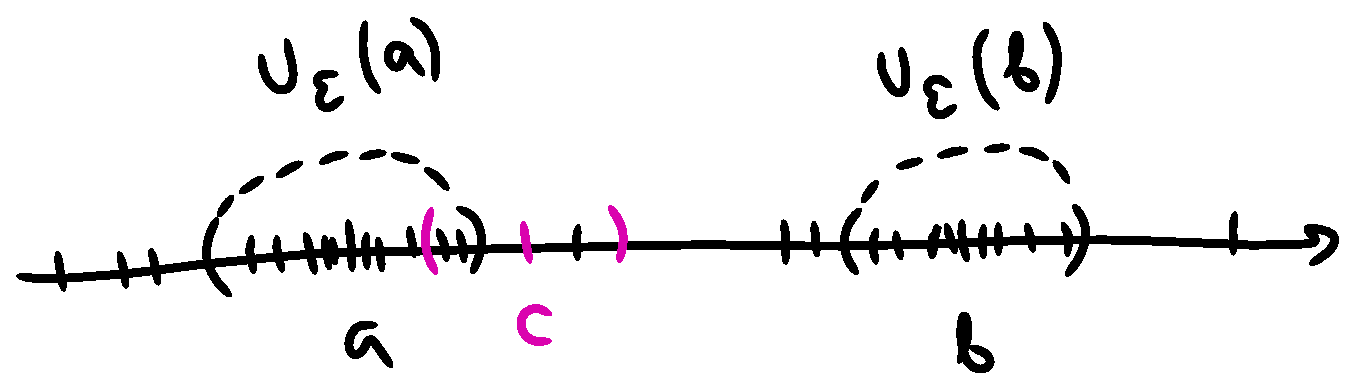
\includegraphics[width=0.6\linewidth]{images/c-somewhere}
      
      \caption{
        Если два частичных предела $a \hm\in \RR$ и $b \hm\in \RR$ не равны, то в любой достаточно малой окрестности любого числа не будет либо бесконечного хвоста подпоследовательности, сходящейся к~$a$, либо бесконечного хвоста подпоследовательности, сходящейся к~$b$.
      }
      \label{fig:c-somewhere}
    \end{figure}
    
    Можно бы было и не думать вообще о расположении~$c$.
    Получим противоречие из условия Коши сходимости $\{x_{3k}\}$.
    По условию Коши, должно быть:
    \[
      \forall \widetilde \eps > 0\ \exists N\colon \forall p, q \geq N \to |x_{3p} - x_{3q}| < \widetilde \eps
    \]
    Но при наличии ``зазора'' между $\eps$-окрестностями $a$ и~$b$ разности между элементами из этих окрестностей будут не меньше ``зазора'', поэтому для $\widetilde \eps$, равного ``зазору'' (то есть снова можно взять $\widetilde \eps \hm= (b \hm- a) \hm/ 4$), условие Коши сходимости для $\{x_{3k}\}$ выполняться не будет (всегда можно будет найти, например, $x_{3p}$ с каким угодно большим чётным номером и $x_{3q}$ с каким угодно большим нечётным).
  \end{solution}
  
\end{document}
